\scanpage{92}
% manuscript lines 1
\uline{Un exemple} [sur un corps alg. clos si on veut

% manuscript lines 1–2
\margin{Où la \deleted{\unsure{co}}\unsure{codim|dim} des lieux des pts non coh. Mac. fait un saut dans la mauvaise direction\ldots\ldots}

% manuscript lines 3–7
\deleted{$A$} $X'$ schéma local \deleted{\unsure{intègre}} \deleted{\unsure{intègre}} \inserted{intègre} de \deleted{profondeur \unsure{de dim} \unsure{$n'$}, \unsure{prof $\geq2$}} \inserted{dim $n'$} \deleted{\unsure{pureté}} \inserted{\unsure{i.e. de prof $1$|i.e. coprof $1$}} (centre $x$) \deleted{contenant une partie $\unsure{Z_1}$ irréductible \uline{$Z_1\ne X$}, telle que \uline{en les pts de $Z_1$}, \uline{$X'$ ne soit} pas \uuline{Cohen-Macaulay}. On a donc $\operatorname{codim}_X Z_1=$} $Z'_0$ \unsure{l'ens|l'un} des pts où \unsure{il} n'est pas Coh. Mac., \inserted{on suppose $Z'_0\ne\{x\}$ \deleted{\illegible{1}}}

% manuscript lines 8–9
$X''$ schéma local \deleted{\unsure{intègre}} \inserted{intègre} de \deleted{\uline{dim} $\unsure{n''}$, $\operatorname{prof}\unsure{\geq}$} \inserted{dim $n''>n'$} $Z''_0$ \unsure{l'ens|l'un} des pts où il n'est pas Coh. Mac.

% manuscript lines 7–10
\figure{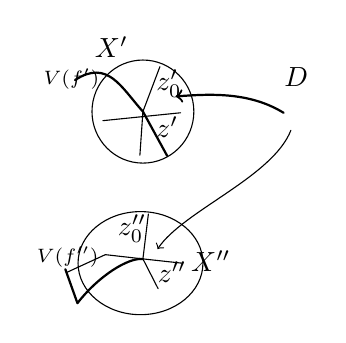
\begin{tikzpicture}[scale=.77,line join=round,line cap=round]
\draw (0,1.5) ellipse (.84 and .85); \node at (-.52,2.56){$X'$};
\draw[thick](-1.12,2.02)..controls(-.58,2.37)and(-.36,1.9)..(0,1.5)--(.4,.77);
\draw (0,1.5)--(.28,2.24) (0,1.5)--(-.05,.78) (-.66,1.35)--(.62,1.48);
\node at (.43,1.96){$z'_0$};\node at (.4,1.25){$z'$};\node at (-1.18,2.04){\scriptsize $V(f')$};
\draw (-.04,-1) ellipse (1.03 and .85); \draw (-1.25,-1.15)--(-.62,-.86)--(0,-.93)--(.64,-1);
\draw[thick](-1.28,-1.1)--(-1.08,-1.66)..controls(-.73,-1.21)and(-.25,-.91)..(0,-.93);
\draw (0,-.93)--(.09,-.19) (0,-.93)--(.25,-1.42);
\node at (-.18,-.43){$z''_0$};\node at (.48,-1.15){$z''$};\node at (1.12,-.96){$X''$};\node at (-1.24,-.9){\scriptsize $V(f'')$};
\node at (2.53,2.07){\uline{$D$}}; \draw[->,thick](2.32,1.48) .. controls (1.75,1.83) and (1.1,1.79) .. (.54,1.75);
\draw[->](2.44,1.19)..controls(2.14,.42)and(.66,-.14)..(.24,-.77);
\end{tikzpicture}}

% manuscript lines 10–11
$D$ un \deleted{\unsure{sous-}}schéma \deleted{fermé de $X$} \inserted{local intègre} de dim $1$

% manuscript lines 12
\deleted{$D'$ \rule{10em}{.35pt} $Y$ de dim $1$}

% manuscript lines 13–14
\[
\left.\begin{aligned}
u' &:D\longrightarrow X'\\
u'' &:D\longrightarrow X''
\end{aligned}\right.\qquad\text{des \uuline{immersions fermées}}
\]

% manuscript lines 15
\[
\underline{u'(D)\not\supset Z'_0}
\]

% manuscript lines 16–20
$X=X'\amalg_D X''$ on identifie $X'$ et $X''$ à des sous-schémas fermés, \unsure{donc} $Z'_0,Z''_0$ aussi. On identifie $D$ à un \deleted{$\unsure{Z}$} ss-schéma fermé \deleted{$\unsure{Z}$} de $X$.

% manuscript lines 17–23
\margin{$A'\times_B A''$\quad $\unsure{f_0}$\quad $\underline{f=(f',f'')}$ \quad $0\longrightarrow C\longrightarrow A'\times A''\xrightarrow{u'-u''}B\longrightarrow0$\quad $(g',g'')\in C$\quad $g'=f'h'$, $g''=f''h''$. $(h',h'')\in C$}
% slanted

% manuscript lines 18–20
\diagram{\begin{tikzcd}[ampersand replacement=\&,row sep=tiny,column sep=small]
\&A'\arrow[r]\& B\\ C\arrow[ur]\arrow[r]\&A''\arrow[ur,dash]\&
\end{tikzcd}}

% manuscript lines 21–23
$f_0\in\deleted{\unsure{H^0}}(\underline O_{D,x})$, $f_0\ne0$. On relève $f_0$ en $f',f''$, d'où $f\in\underline O_{X,x}$ \deleted{est} qui est \uline{non div de $0$} \deleted{\unsure{donc}}. On a
\[
 V(f)\simeq V(f')\amalg_{V(f_0)}V(f'')
\]
% archive sheet number: 91

